\chapter{Sicherheitseigenschaften}
\label{SK}

In diesem Kapitel werden Begriffe eingeführt, welche die Sicherheit kryptographischer Verfahren formalisieren. Diese Sicherheitseigenschaften sind Kriterien, anhand derer ein Kryptosystem bewertet wird.

Die Sicherheitsbegriffe für Kryptosysteme, welche jetzt vorgestellt werden, lassen sich grundsätzlich wie folgt einteilen:

\begin{itemize}
	\item Sicherheitsbegriffe, die \textit{Angreifermodelle} definieren 
	\item Sicherheitsbegriffe, die ein wünschenswertes \textit{Sicherheitsziel} definieren
\end{itemize}

Diese Einteilung wurde ursprünglich von Moni Noar vorgeschlagen\footnote{Dies wird in \cite{bellare1998relations} erwähnt und hier wird eine Quelle zitiert welche nicht ausfindig gemacht werden konnte: M. Noar, private communication, März 1998. Diese Aufteilung findet sich jedoch auch so in \cite[p.289]{smart2003}: Notions of security, Notions of attacks.}.

Betrachtet man ein asymmetrisches Kryptosystem, bei dem der öffentliche Schlüssel bekannt ist, so ermöglicht dies einem Angreifer jeden beliebigen Klartext unter diesem Schlüssel zu verschlüsseln. Diese Fähigkeit des Angreifers führt zu dem Angreifermodell \textit{Adaptiver Angriff mit ausgewähltem Klartext} in Abschnitt \ref{angreifermodelle}. Ein zu erreichendes Sicherheitsziel bei einem Kryptosystem ist die Vermeidung einer \textit{Verformung von Chiffretexten durch unautorisierte Dritte}, welches in Abschnitt \ref{malleability} definiert wird.

\section{Angreifermodelle der Kryptoanalyse}
\label{angreifermodelle}

Angriffe auf ein Kryptosystem versuchen die vertrauliche Information, den verschlüsselten Klartext, aus einem Chiffretext zu rekonstruieren oder den eingesetzten Schlüssel zu rekonstruieren.

Bei der Beurteilung der Sicherheit von kryptographischen Verfahren geht man in der modernen Kryptoanalyse davon aus, dass der Angreifer die Algorithmen kennt, welche ein Kryptosystem einsetzt. Dieser Gedanke wurde von Shannon erstmals formuliert \cite[p.662]{shannon1949communication}. Damit soll die Sicherheit eines Kryptosystems nur von dem Schlüssel abhängen, was auch als das Kerckhoffsche Prinzip bekannt ist.

Im Folgenden werden verschiedene Angreifermodelle der Kryptoanalyse vorgestellt. Diese unterscheiden sich dadurch, auf welche Informationen der Angreifer zurückgreifen kann, um Informationen aus Chiffraten zu gewinnen. Dabei betrachten wir diejenigen Angreifermodelle, welche für asymmetrische Verfahren relevant sind. %: Bei Asymmetrischen Verfahren ist der öffentliche Schlüssel in der Regel dem Angreifer bekannt und ermöglicht ihm so beliebige willkürliche Klartexte unter dem Verschlüsselungsalgorithmus des Kryptosystem zu verschlüsseln, welches ihm ebenso bekannt ist. 

Die Angreifermodelle werden in der Reihenfolge nach der Stärke des Angreifers vorgestellt, angefangen mit dem schwächsten \cite[p.4-5]{delfs2002introduction}\cite[p.7-8]{beutelspacher1995moderne}:

\textbf{Reiner Chiffretext-Angriff (\textit{ciphertext-only attack}/COA):}
Bei dieser Angriffsform ist der Angreifer in der Lage Zugriff auf Chiffretexte einer vertraulichen Kommunikation zu bekommen. Den Chiffretext kann sich der Angreifer nicht auswählen, da er nicht in die Kommunikation eingreift. Bei einem reinen Chiffretext-Angriff handelt es sich um die schwächste Form eines Angreifers. Kann ein Angreifer ohne Aufwand unter diesem Angreifermodell Einsicht in die verborgenen Klartexte gelangen, so bietet das Kryptosystem keinen Schutz - es ist unsicher.

\textbf{Angreifer mit bekannten Klartext (\textit{known-plaintext attack}/KPA):}
Der Angreifer hat Zugriff auf eine begrenzte Zahl aus Chiffretexten und zugehörigen Klartexten. Anhand der Beziehungen welche zwischen den Klartext-Chiffretext-Paaren besteht, versucht der Angreifer Kenntnisse über die Algorithmen des Kryptosystems zu gewinnen. Mit den gewonnenen Erkenntnissen versucht er dann Chiffretexte zu entschlüsseln, für welche kein passender Klartext vorliegt. Dieser Angriff ist möglich in Situationen, in welchen im Klartext mit standardisierten Formaten kommuniziert wird. So beginnen z.B. PDF-Dateien im Header mit einem fest definierten String, z.B. \enquote{\%PDF-1.7}. Dieser gibt die Version des Portable Document Formats an \cite[p.92]{pdfrefer40:online}. Im zweiten Weltkrieg wurde Enigma mit bekannten Klartexten angegriffen \cite{schneier2011secrets}.

\textbf{Angreifer mit ausgewählten Klartext (\textit{chosen-plaintext attack}/CPA1):}
Der Angreifer ist in der Lage \textit{einmal} Chiffretexte zu einer Menge ausgewählter Klartexte zu erzeugen. Information die daraus gewonnen werden kann, wird benutzt um unbekannte Chiffretexte zu entschlüsseln. Es ist dem Angreifer insbesondere nicht möglich, die Ergebnisse der Analyse eines Klartext-Chiffretext-Paars zu benutzten um ein weiteres Paar zu erzeugen. Alle Paare erhält der Angreifer am Anfang des Angriffs zusammen. Im Falle von asymmetrischen homomorphen Kryptosystemen muss dieses Angreifermodell grundsätzlich betrachtet werden, da der öffentliche Schlüssel frei verfügbar ist. Damit hat ein Angreifer eines asymmetrischen homomorphen Kryptosystems \textit{immer} die Möglichkeit ausgewählte Klartexte anzugreifen. 

\textbf{Adaptiver Angreifer mit ausgewählten Klartext (\textit{adaptive chosen-plaintext attack}/CPA2):}
Dieses Angreifermodell ist eine Erweiterung des  Angriffs mit ausgewähltem Klartext. Dabei kann der Angreifer nach Erhalt eines Klartext-Chiffretext-Paares ein weiteres erzeugen und dabei Information aus der Analyse des vorherigen Klartext-Chiffretext-Paares ausnutzen. Damit ist dieser Angriff im Vergleich zu CPA1 \textit{interaktiv}. Der Angreifer hat Zugriff zu einem Verschlüsselungsapparat\footnote{Verschlüsselungs- und Entschlüsselungsapparate sind Funktionen die dem Angreifer ermöglichen Klartexte zu verschlüsseln und Chiffretexte zu entschlüsseln, in deren Funktionsweise der Angreifer jedoch keine Einsicht hat.  Daher spricht in der Literatur auch von einer Black Box \cite[p.291]{smart2003} oder einem Entschlüsselungsorakel \cite[p.2]{bellare1998relations}.} oder kann diesen mehrmals verwenden.

\textbf{Angreifer mit ausgewählten Chiffretext (\textit{chosen-ciphertext attack}/CCA1):}
Analog zu CPA1 definiert man: Der Angreifer hat \textit{einmal} Zugriff zu Klartexten von ausgewählten Chiffretexten durch einen Entschlüsselungsapparat. Bleichenbacher präsentiert in \cite{bleichenbacher1998chosen} einen Angriff mit ausgewählten Chiffretexten, der erfolgreich ein RSA-basiertes Protokoll aus dem SSL 3.0 Standard bricht.

\textbf{Adaptiver Angreifer mit ausgewählten Chiffretext (\textit{adaptive chosen-ciphertext attack}/CCA2):}
Wie bei dem Angreifermodell in CPA2 ist der Angriff interaktiv. Der Angreifer kann Klartexte zu ausgewählten Chiffretexten erhalten und anschließend erneut mit dem Entschlüsselungsapparat einen weiteren Chiffretext entschlüsseln.
Bei dem Schutz vor adaptiven Angriffen mit ausgewählten Chiffretexten handelt es sich um die stärkste mögliche Anforderung an ein Kryptosystem.

\subsection{Anmerkungen zu den Angreifermodellen} 

In der Literatur werden diese Angriffe in passive und aktive Angreifermodelle unterteilt. Jedoch führen die Definitionen zu verschiedenen Aufteilungen: Buchmann unterscheidet Angreifer danach, ob sie nur Chiffretexte (passiv) oder gleichzeitig ausgewählte Klartexte und Chiffretexte (aktiv) angreifen können \cite[p.76]{buchmann2004introduction}. Smart dagegen bezeichnet in \cite[p.291]{smart2003} den Angriff mit ausgewähltem Klartext als passiv.

Statt der Angreifermodelle CPA1 und CPA2 ist der Gebrauch der Bezeichnung CPA üblich  \cite{armknecht2013group}. Damit ist CPA2-Sicherheit gemeint, da die Verschlüsselungsfunktionen der eingesetzten Kryptosysteme bekannt sind. Die Kryptosysteme, welche in dieser Bachelorarbeit behandelt werden, sind öffentlich bekannt. Daher wird im weiteren Verlauf nur von CPA-Sicherheit gesprochen, um die Angreifermodelle CPA1 und CPA2 gleichermaßen abzudecken.

\section{Sicherheitszeile}

Im Folgenden wird formalisiert, inwiefern ein Angreifer Einsicht in Chiffretexte erhält durch Angabe seines Vorteils (engl. \textit{advantage}) gegenüber einem ratenden Angreifer. 

\subsection{Perfekte Sicherheit}

In einem Kryptosystem mit perfekter Sicherheit (engl. \textit{perfect security}) ist es für einen Angreifer mit unendlich großer Rechenkapazität nicht möglich, etwas über den Klartext anhand eines vorliegenden Klartextes zu lernen. 

\begin{theorem}[Perfekt Sicheres Kryptosystem]
Sei $K = (\mathcal{P},\mathcal{C},\mathcal{K},\mathcal{E},\mathcal{D})$ ein Kryptosystem. Dann ist K perfekt sicher, wenn für alle $x\in\mathcal{P}$ und alle $c\in\mathcal{C}$ gilt:
\begin{equation*}
\text{Pr}(P=x\ |\ C=c) = \text{Pr}(P=x).
\end{equation*}

\end{theorem}

\cite[p.280]{smart2003}

 Laut dem Theorem von Shannon ist dies genau dann der Fall, wenn 1) alle Schlüssel $k\in\mathcal{K}$ des Schlüsselraums gleichverteilt gezogen werden und 2) jeder Schlüssel nur einmal verwendet wird. \cite[p.36]{katz2014introduction} Aus diesem Grund sind asymmetrische Kryptosysteme im praktischen Einsatz nicht perfekt sicher, da man den gleichen Schlüssel für mehrere Klartexte verwendet.
 
\subsection{Semantische Sicherheit}
\label{semantischSicher}

Der Begriff semantischer Sicherheit (engl. \textit{semantic security}) unterscheidet sich von perfekter Sicherheit darin, dass die Rechenkapazitäten des Angreifers nach oben polynomiell beschränkt sind \cite[p.290]{smart2003}
\cite[p.166]{buchmann2004introduction}.

Auf eine formale Definition wird in diesem Abschnitt verzichtet, denn semantische Sicherheit ist gleichbedeutend zu der Unterscheidbarkeit von Chiffretexten \cite[p.8]{goldreich1993uniform}\cite[p.203]{delfs2002introduction}. Diese wird im nächsten Abschnitt eingeführt.

\subsection[Ununterscheidbarkeit von Chiffretexten (ciphertext indistinguishability/IND)]{\texorpdfstring{Ununterscheidbarkeit von Chiffretexten\\ (ciphertext indistinguishability/IND)}{Ununterscheidbarkeit von Chiffretexten (ciphertext indistinguishability/IND)}}
\label{IND}

Gegeben zwei Klartexte $x_1, x_2$ und ein Chiffretext $c_b$ von einem der beiden Klartexte bedeutet Unterscheidbarkeit von Chiffretexten (engl. \textit{ciphertext indistinguishability}, kurz: IND), dass es einem Angreifer $\mathcal{A}$ nicht möglich ist $c_b$ dem zugehörigen Klartext zuzuordnen. Damit meint man, dass der Angreifer diese Zuordnung mit einer Wahrscheinlichkeit treffen muss, die größer ist, als wenn er zufällig raten würde (hier: $>\frac{1}{2}$). Es wird dem Angreifer jedoch erlaubt, die Länge des Klartextes anhand des Chiffretextes zu lernen. Daher wird im Folgenden vorausgesetzt, dass die Klartexte $x_1, x_2$ immer die gleiche Länge haben \cite[p.32]{bellare1998relations}. 

Wäre das verwendete Kryptosystem deterministisch, so würde dem Angreifer diese Zuordnung durch Evaluierung der Verschlüsselungsfunktion gelingen. Mit dem öffentlichen Schlüssel $k_p$ berechnet der Angreifer $c_i = e_{k_p}(x_i)$. Durch einen Vergleich mit dem erhaltenen Chiffretext $c_b$ kann der Angreifer $b$ bestimmen. Daher muss bei einem IND-sicherem Kryptosystemen die Verschlüsselungsfunktion probabilistisch sein, denn sonst gelingt dem Angreifer diese Zuordnung.
%RSA ohne Padding ist nicht IND-Sicher 

Formalisiert wird die Ununterscheidbarkeit von Chiffretexten als ein Spiel, das der Angreifer spielt. Der Vorteil des Angreifers wird angegeben als die Differenz der Wahrscheinlichkeit mit der der Angreifer $c_b$ dem richtigen $x_i$ zuordnen kann, und der Erfolgswahrscheinlichkeit eines zufällig ratenden Angreifers.

Sei $\mathcal{A}$ ein Angreifer. Dann lässt sich der Angriff als ein Spiel in zwei Schritten auffassen:

\begin{enumerate}
	\item Im ersten Schritt erzeugt der Angreifer zwei Klartexte $x_1, x_2$. 
	\item Im zweiten Schritt erhält der Angreifer $\mathcal{A}$ das anzugreifende Chiffrat:\\
	Sei $c_b$ die Verschlüsselung von einem der beiden Klartexte. Das Ziel von $\mathcal{A}$ ist nun  den geheimen Wert $b$ mit einer Wahrscheinlichkeit $>\frac{1}{2}$ zu ermitteln.
\end{enumerate}

Dies führt zu dem Vorteil $\text{Adv}_\mathcal{A}$ des Angreifers \cite[p.291]{smart2003}:
\begin{equation*}
\text{Adv}_\mathcal{A} = \left| Pr\left(\mathcal{A}(\text{ermitteln},c_b,k_p,x_1,x_2)=b\right)-\frac{1}{2}  \right|.
\end{equation*}

Dabei steht \enquote{Adv} für Advantage. Weiter nennt man das Kryptosystem polynomiell sicher (engl. \textit{polynomially secure}), wenn die Wahrscheinlichkeit des Ratens für Angreifer beschränkt ist durch:

\begin{equation*}
\text{Adv}_\mathcal{A}  \leq \frac{1}{p(n)}.
\end{equation*}

Mit beliebigen Polynomen $p$ vom Grad $n$. Man nennt den Vorteil des Angreifers dann vernachlässigbar klein.

Diese Formalisierung der Ununterscheidbarkeit von Chiffretexten kann erweitert werden auf die in Abschnitt \ref{angreifermodelle} vorgestellten Angreifermodelle. Man spricht dann z.B. von einer Ununterscheidbarkeit von Chiffretexten bei einem Angreifer auf bekannten Klartext (engl.: \textit{indistinguishability under chosen-ciphertext attack}/IND-CPA). Weiter: IND-CCA1, IND-CCA2 \cite[p.33]{bellare1998relations}. Oft wird nur von semantischer Sicherheit eines Kryptosystems gesprochen. Hiermit ist IND-CPA-Sicherheit gemeint, da kein Angreifer mit Entschlüsselungsapparat betrachtet wird \cite[p.27]{dolev2003nonmalleable}.

\subsection[Keine unautorisierte Verformbarkeit von Chiffretexten (non-malleability/NM)]{\texorpdfstring{Keine unautorisierte Verformbarbarkeit von Chiffretexten\\ (non-malleability/NM)}{Keine unautorisierte Verformbarkeit von Chiffretexten (non-malleability/NM)}}
\label{malleability}

Im Folgenden wird zur Definition von \enquote{keine unautorisierte Verformbarkeit von Chiffretexten} (engl. \textit{non-malleability}, kurz: NM) zum besseren Verständnis zunächst folgende intuitive Idee vorgestellt:
Ein Kryptosystem das nicht NM-sicher ist, hat folgende Eigenschaft: Ein Angreifer kann einen Chiffretext $c$ von Klartext $x$ gezielt verformen, um einen daraus abgeleiteten Chiffretext $c'$ zu erzeugen, welcher in einer ihm bekannten Beziehung zu $c$ steht \cite[p.292]{smart2003}.

Während die Ununterscheidbarkeit von Chiffretexten formalisiert, dass ein Angreifer aus einem Chiffretext nichts über den Klartext lernt, formalisiert NM, dass ein Angreifer aus einem Chiffretext keinen angeleiteten Chiffretext erzeugen kann.

Man betrachte das Szenario einer Versteigerung, welche die Partei $\mathcal{R}$ leitet. Teilnehmende Bieter sind die Parteien $\mathcal{S}$ und $\mathcal{A}$. Ihre Gebote geben sie an $\mathcal{R}$ verschlüsselt unter dem öffentlichen Schlüssel von $\mathcal{R}$ ab. Verwendet wird das Kryptosystem von Okamoto-Uchiyama. Dieses erlaubt eine homomorphe Addition zu einem Chiffretext mit dem öffentlichen Schlüssel. Dann könnte $\mathcal{A}$ folgenden Angriff durchführen:
\begin{enumerate}
	\item $\mathcal{A}$ wartet bis $\mathcal{S}$ sein verschlüsseltes Gebot $c$ abgibt. Der zugehörige Klartext $x$ ist $\mathcal{A}$ nicht bekannt.
	\item Dann fängt $\mathcal{A}$ das Gebot $c$ von $\mathcal{S}$ ab und erzeugt ein eigenes Gebot $c'$, dessen Klartext $x'$ das um $1$ erhöhte Gebot von $x$ ist: $x'=x+1$.
\end{enumerate} 
Somit gewinnt $\mathcal{A}$ die Auktion. Beispiel entnommen aus \cite[p.388]{katz2014introduction}.

In der Literatur finden sich verschiedene formale Definitionen für NM-Sicherheit von \cite[p.34]{bellare1998relations}\cite[p.12]{dolev2003nonmalleable} von denen Bellare et al. \cite{bellare1999non} beide als äquivalent nachgewiesen hat. Hier wird die Definition von Dolev \cite{bellare1998relations} vorgestellt:

Zunächst zur Notation: 
Sei $X\notin\perp$ eine nicht-leere Menge von Klartexten und $x\in X$ ein zu $X$ zugehöriger Klartext. Dann bezeichnet $X\leftarrow\mathcal{D}_{k_s}(C)$ die Entschlüsselung aller Chiffretexte $c\in C$. Es werden t-stellige Relationen betrachtet. Anstelle von $R(x_1,\ldots,x_t)$ wird $R(x,X)$ notiert, wo bei $x$ ein gesonderter Klartext und $X$ eine Menge mit $t-1$ Klartexten ist.

Der Angreifer hat nun zum Ziel zu einem Chiffretext $c$ mit der Entschlüsselung $x$ eine Menge abgeleiteter Chiffretexte $C$ zu erzeugen, deren Entschlüsselung  $X$ zu $x$ in einer Relation $\mathcal{R}(x,X)$ steht.

Das Sicherheitsziel wird durch ein Spiel beschrieben, das der Angreifer spielt. Dabei wird das Kryptosystem als sicher bewertet, wenn der Angreifer nicht besser abschneidet als ein ratender Angreifer. Die Differenz der Wahrscheinlichkeiten wird wie schon bei der Ununterscheidbarkeit von Chiffretexten als Vorteil des Angreifers angegeben.

Sei $\mathcal{A} = (\mathcal{A}_1,\mathcal{A}_2)$ ein Angreifer. Formal fasst man seine Aktivitäten in zwei Algorithmen $\mathcal{A}_1,\mathcal{A}_2$, die nacheinander ausgeführt werden. So lässt sich der Angriff als ein Spiel in zwei Schritten beschreiben:
	
\begin{enumerate}
		\item Im ersten Schritt erzeugt der $\mathcal{A}_1$ eine Beschreibung des Klartextraums:\\
		Es wird ein asymmetrisches Kryptosystem angegriffen. Daher hat $\mathcal{A}_1$ Zugriff auf den öffentlichen Schlüssel $k_p$ als Eingabeparameter. $\mathcal{A}_1$ erzeugt nun einen Samplingalgorithmus $M$ aus dem Klartexte $x$ gezogen werden können\footnote{Dieser Schritt dient lediglich als Vorbereitung für den zweiten Schritt. Vergleiche hierzu den ersten Schritt des Angreifers in \ref{IND}. Dort stellt dieser in der Vorbereitungsphase zwei Klartexte zur Verfügung. Von diesen wird eines dem Angreifer verschlüsselt zurückgegeben, welches er angreifen muss. Entsprechend kann hier der Angreifer mit $M$ festlegen welche Klartextnachrichten benutzt werden um ein davon abhängiges Chiffrat zu erzeugen.}.
		\item Im zweiten Schritt erhält $\mathcal{A}_2$ das anzugreifende Chiffrat :\\
		Aus M wird ein Klartext $x$ gezogen, welches der  $\mathcal{A}_2$ nicht kennt. Es wird ihm nur der zugehörige Chiffretext $c\leftarrow\mathcal{E}_{k_s}(x)$ gegeben. Die Herausforderung, welche  $\mathcal{A}_2$ nun bewältigen muss, ist folgende:  $\mathcal{A}_2$ erzeugt eine (Beschreibung der) Relation $\mathcal{R}$ und eine Menge $C\notni c$ von Chiffretexten.  $\mathcal{A}_2$ hofft, dass für die zu $C$ zugehörigen Klartexte $X$ die Relation $R(x,X)$ gilt. Der  $\mathcal{A}_2$ ist erfolgreich, wenn für sein erzeugtes $C$ eine Relation $R(x,X)$ wahrscheinlicher ist als eine Relation $R(\tilde{x},X)$, wobei $\tilde{x}\in M$ ein zufällig gewählter Klartext ist.
		
		Die Wahrscheinlichkeit für das erfolgreiche Schätzen des Angreifers wird als $\text{Succ}^{NM-a}_{A,K}(n)$ notiert.  Die Wahrscheinlichkeit, dass die vom Angreifer erzeuge Relation $R$ und Menge $C$ zu einem zufälligen $\tilde{x}\in M$ passen, wird mit $\text{Succ}^{NM-a}_{A,K,\$}(n)$ notiert.
		
		
\end{enumerate}

\begin{theorem}[Keine unautorisierte Verformbarkeit: NM-CPA, NM-CCA1, NM-CCA2]
\label{DefKuV}
\qquad\qquad\qquad Sei $K = (\mathcal{P},\mathcal{C},\mathcal{K},\mathcal{E},\mathcal{D})$ ein asymmetrisches Kryptosystem und sei $\mathcal{A} = (\mathcal{A}_1,\mathcal{A}_2)$ ein Angreifer. Für $a\in\{CPA,CCA1,CCA2\}$ und $n\in\mathbb{N}$ ist der Vorteil des Angreifers bei NM-$a$:
	
\begin{equation*}
\normalfont
\text{Adv}^{NM-a}_{A,K}(n)= \left| \text{Succ}^{NM-a}_{A,K}(n)-\text{Succ}^{NM-a}_{A,K,\$}(n) \right| 
\end{equation*}	
mit
\begin{align*}
\normalfont
\text{Succ}^{NM-a}_{A,K}(n) =\
& Pr \left(  
(k_p,k_s)\leftarrow\mathcal{K};\
(M,s)\leftarrow A^{\mathcal{O}_1}_1(k_p);\
x\leftarrow M;\
c\leftarrow\mathcal{E}_{k_s}(x); \right.\\
& \left.  (R,C)\leftarrow A^{\mathcal{O}_2}_2(M,c,s);\
\textbf{x}\leftarrow\mathcal{D}_{k_s}(C) : c\notin C \wedge \perp\notni X \wedge R(x,X)  \right)
\end{align*}		
\begin{align*}
\normalfont
\text{Succ}^{NM-a}_{A,K,\$}(n) =\
& Pr\left( 
(k_p,k_s)\leftarrow\mathcal{K};\
(M,s)\leftarrow A^{\mathcal{O}_1}_1(k_p);\
x,\tilde{x}\leftarrow M;\
c\leftarrow\mathcal{E}_{k_s}(x); \right.\\
& \left. (R,C)\leftarrow A^{\mathcal{O}_2}_2(M,c,s);\
X\leftarrow\mathcal{D}_{k_s}(C) : c\notin C \wedge \perp\notni X\wedge R(\tilde{x},X)
\right).
\end{align*}
Wobei je nach Angreifermodell für den Entschlüsselungsapparat $\mathcal{O}$ gilt:
\begin{alignat*}{3}
&\normalfont\text{Wenn}\ a=CPA, \ &&\normalfont\text{dann ist}\ \mathcal{O}_1(\cdot)= \epsilon\ &&\normalfont\text{und}\ \mathcal{O}_2(\cdot) = \epsilon.\\
&\normalfont\text{Wenn}\ a=CCA1, \ &&\normalfont\text{dann ist}\ \mathcal{O}_1(\cdot)=\mathcal{D}_{k_s}(\cdot)\ &&\normalfont\text{und}\ \mathcal{O}_2(\cdot) = \epsilon.\\
&\normalfont\text{Wenn}\ a=CCA2, \ &&\normalfont\text{dann ist}\ \mathcal{O}_1(\cdot)=\mathcal{D}_{k_s}(\cdot)\ &&\normalfont\text{und}\ \mathcal{O}_2(\cdot) = \mathcal{D}_{k_s}(\cdot).\\
\end{alignat*}
\end{theorem}
Im Falle des CPA Angreifermodells gibt es keinen Entschlüsselungsapparat. Daher ist der Entschlüsselungsapparat das leere Wort. Im Falle des CCA1 Angreifermodells kann der Angreifer nach Analyse seiner Klartext-Chiffretext-Paare nicht erneut den Entschlüsselungsapparat anfragen, daher ist $\mathcal{O}_2$ das leere Wort. Im Falle des CCA2 Angreifermodells wird vorausgesetzt, dass der Angreifer den Entschlüsselungsapparat nicht anfragt den Chiffretext $c$ zu entschlüsseln.

Bei dem Parameter $s$ handelt es sich um Zustandsinformationen des Algorithmus $\mathcal{A}_1$ die an  $\mathcal{A}_2$ weitergegeben werden kann (wie z.B. den öffentlichen Schlüssel). Bellare et al. benötigen diesen Parameter für ihre Beweise von Implikationen zwischen den Sicherheitskriterien, welche im nächsten Abschnitt erläutert werden. 

Sei die Rechenkapazität des Angreifers $\mathcal{A} = (\mathcal{A}_1,\mathcal{A}_2)$ polynomiell durch $p(n)$ beschränkt, mit Polynom $p$ und $n\in\mathbb{N}$. Ein Kryptosystem wird NM-a-sicher genannt ($a\in\{CPA,CCA1,CCA2\}$), wenn der Vorteil des Angreifers beschränkt ist durch:
\begin{equation*}
	\text{Adv}^{NM-a}_{A,K}(n) \leq \frac{1}{p(n)}.
\end{equation*}

%Das Kryptosystem $K$ gilt dann als $NM-a$ sicher, wenn der Angreifer zu Ausführung aller seiner Schritte


\section{Implikationen zwischen den Sicherheitskriterien} 
\label{impli}

Angreifermodelle und Sicherheitsziele wurden in vorherigen Abschnitten zu den Sicherheitskriterien IND-CPA/NM-CPA, IND-CCA1/NM-CCA1 und IND-CCA2/NM-CCA2 zusammengefasst. Da diese Definitionen teilweise Erweiterungen voneinander sind, existieren zwischen ihnen Implikationen: So impliziert CCA2-Sicherheit einen Schutz gegenüber dem schwächeren Angreifermodell CCA1, was direkt aus der Definition in \ref{angreifermodelle} folgt.

Darüber hinaus gibt es weitere Implikationen, welche in \cite{bellare1998relations} alle bewiesen wurden. Dies führt zu folgenden Beziehungen zwischen den Sicherheitskriterien:
\begin{figure}[h]
	\begin{center}
		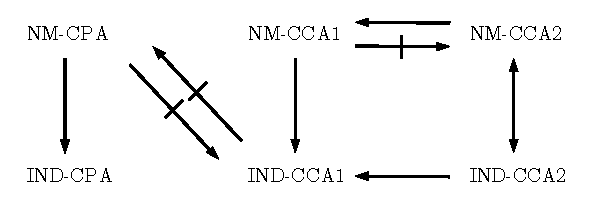
\includegraphics{fig/Implikationen}
		\caption{Implikationen zwischen Sicherheitskriterien kryptografischer Verfahren. Ein Pfeil bedeutet, dass diese Implikation formal bewiesen wurde. Ein durchgestrichener Pfeil bedeutet, dass diese Implikation als ungültig bewiesen wurde.}
		\label{fig:plots}
	\end{center}
\end{figure}

Unter dem gleichen Angreifermodell impliziert also NM-Sicherheit immer auch IND-Sicherheit. 

\section{Private Datenverarbeitung}
\label{privacypreserving}
Mehrere der in Kapitel \ref{KHK} vorgestellten Studien setzen homomorphe Kryptosysteme zur Wahrung der Privatsphäre der hinterlegten Daten ein (engl. \textit{privacy preserving}). Mit Datenverarbeitung unter Wahrung der Privatsphäre wird verstanden, dass die Daten unter einem Kryptosystem verschlüsselt sind, das eines der hier vorgestellten Sicherheitskriterien erfüllt.

\section{Honest-but-curious Angreifermodell}
\label{hbc}

\textit{Honest-but-curious} (HBC) ist ein Angreifermodell für Protokolle in denen mehrere Parteien kooperieren. In einem Angriff werden eine oder mehrere Parteien, die am Protokoll teilnehmen, von dem Angreifer übernommen. Der Angreifer hat dann Zugriff auf alle Daten, welche die Partei sehen kann. Der Angreifer ist ehrlich (engl. \textit{honest}) und hält sich an das Protokoll. Er versucht jedoch die Daten, welche er lesen kann, aus Neugierde zu analysieren (engl. \textit{curious}). Mehrere vom Angreifer übernommene Parteien können kooperieren, um Sicherheitsgarantien des Protokolls zu umgehen. Ist ein Protokoll sicher bzgl. des honest-but-curious Angreifermodells, werden folgende Annahmen gemacht:
\begin{enumerate}
	\item Der Angreifer ist honest-but-curious.
	\item Sei n die Anzahl der am Protokoll beteiligen Partien. Dann werden höchstens n/2 Parteien vom Angreifer übernommen.
\end{enumerate}
In dieser Arbeit verfügen die honest-but-curious Angreifer darüber hinaus über polynomiell beschränkte Rechenkapazitäten. Damit sind sie nicht in der Lage die eingesetzten Kryptosysteme zu brechen.
Neben honest-but-curious Angreifern betrachtet man \textit{bösartige} Angreifer (engl. \textit{malicious}). Bösartige Angreifer dürfen vom Protokoll abweichen und dürfen insbesondere keine Daten oder inkorrekte Daten senden  \cite[p.385]{smart2003}.